\problemname{Radio Towers}

\begin{quote}
\textit{Note:} in this problem, you have to write your solution in C++.
\end{quote}

There are $N$ radio towers in Jakarta. The towers are located along a straight line and numbered
from $0$ to $N-1$ from left to right. For each $i$ such that $0 \leq i \leq N-1$, the height of tower
$i$ is $H[i]$ metres. The heights of the towers are distinct.

For some positive interference value $\delta$, a pair of towers $i$ and $j$ (where
$0 \leq i < j \leq N-1$) can communicate with each other if and only if there is an intermediary
tower $k$, such that
\begin{itemize}
  \item tower $i$ is to the left of tower $k$ and tower $j$ is to the right of tower $k$, that is,
  $i < k < j$, and
  \item the heights of tower $i$ and tower $j$ are both at most $H[k] - \delta$ metres.
\end{itemize}

Pak Dengklek wants to lease some radio towers for his new radio network. Your task is to answer $Q$
questions of Pak Dengklek which are of the following form: given parameters $L$, $R$ and $D$
($0 \leq L \leq R \leq N-1$ and $D > 0$), what is the maximum number of towers Pak Dengklek can
lease, assuming that
\begin{itemize}
  \item Pak Dengklek can only lease towers with indices between $L$ and $R$ (inclusive), and
  \item the interference value $\delta$ is $D$, and
  \item any pair of radio towers that Pak Dengklek leases must be able to communicate with each
  other.
\end{itemize}

Note that two leased towers may communicate using an intermediary tower $k$, regardless of whether
tower $k$ is leased or not.

\section*{Implementation Details}
You should implement the following procedures:

\begin{verbatim}
void init(int N, std::vector<int> H)
\end{verbatim}

\begin{itemize}
  \item $N$: the number of radio towers.
  \item $H$: an array of length $N$ describing the tower heights.
  \item This procedure is called exactly once, before any calls to \texttt{max\_towers}.
\end{itemize}

\begin{verbatim}
int max_towers(int L, int R, int D)
\end{verbatim}

\begin{itemize}
  \item $L$, $R$: the boundaries of a range of towers.
  \item $D$: the value of $\delta$.
  \item This procedure should return the maximum number of radio towers Pak Dengklek can lease for
  his new radio network if he is only allowed to lease towers between tower $L$ and tower $R$
  (inclusive) and the value of $\delta$ is $D$.
  \item This procedure is called exactly $Q$ times.
\end{itemize}

Your submission must not contain a \texttt{main} function, and must not read from standard input or
write to standard output: a grader is compiled together with your submission and does that for you.
The declarations above live in \texttt{towers.h}, which is available both to your submission and as
an attachment, so start your file with \texttt{\#include "towers.h"}.

The judge reveals one question at a time and waits for its answer before revealing the next one, so
\texttt{max\_towers} cannot see the questions that come after it.

\section*{Constraints}
\begin{itemize}
  \item $1 \leq N \leq 10^5$
  \item $1 \leq Q \leq 10^5$
  \item $1 \leq H[i] \leq 10^9$ (for each $i$ such that $0 \leq i \leq N-1$)
  \item $H[i] \neq H[j]$ (for each $i$ and $j$ such that $0 \leq i < j \leq N-1$)
  \item $0 \leq L \leq R \leq N-1$
  \item $1 \leq D \leq 10^9$
\end{itemize}

\section*{Scoring}
Your solution will be tested on a set of test groups.
To earn points for a group, you must pass all test cases in that group.

\noindent
\begin{tabular}{| l | l | p{12cm} |}
  \hline
  \textbf{Group} & \textbf{Points} & \textbf{Constraints} \\ \hline
  $1$ & $4$  & There exists a tower $k$ ($0 \leq k \leq N-1$) such that $H[i] < H[i+1]$ for each $i$
               with $0 \leq i \leq k-1$, and $H[i] > H[i+1]$ for each $i$ with
               $k \leq i \leq N-2$. \\ \hline
  $2$ & $11$ & $Q = 1, N \leq 2000$ \\ \hline
  $3$ & $12$ & $Q = 1$ \\ \hline
  $4$ & $14$ & $D = 1$ \\ \hline
  $5$ & $17$ & $L = 0, R = N-1$ \\ \hline
  $6$ & $19$ & The value of $D$ is the same in all questions. \\ \hline
  $7$ & $23$ & No additional constraints. \\ \hline
\end{tabular}

\section*{Sample Grader}
A sample grader is available under ``attachments'' at the bottom of this page, together with
\texttt{towers.h} and the sample input. Compile it with your solution and run it on an input file to
try your solution locally. It reads the input in the following format:
\begin{itemize}
  \item line $1$: $N$ $Q$
  \item line $2$: $H[0]$ $H[1]$ $\ldots$ $H[N-1]$
  \item line $3 + j$ ($0 \leq j \leq Q-1$): $L$ $R$ $D$ for question $j$
\end{itemize}
and prints the $Q$ return values of \texttt{max\_towers}, one per line. That is the format of the
sample data below.

\section*{Explanation of Sample}
The sample data corresponds to the following sequence of calls:

\begin{center}
\begin{tabular}{| l | l |}
  \hline
  \textbf{Call} & \textbf{Return value} \\ \hline
  \texttt{init(7, [10, 20, 60, 40, 50, 30, 70])} & \\ \hline
  \texttt{max\_towers(1, 5, 10)}  & $3$ \\ \hline
  \texttt{max\_towers(2, 2, 100)} & $1$ \\ \hline
  \texttt{max\_towers(0, 6, 17)}  & $2$ \\ \hline
\end{tabular}
\end{center}

\noindent
In the sample, the heights are $H = [10, 20, 60, 40, 50, 30, 70]$.

For question $0$, with $L = 1$, $R = 5$ and $D = 10$, Pak Dengklek can lease towers $1$, $3$ and $5$.
This is illustrated in the following picture, where shaded trapezoids represent leased towers.

\begin{center}
  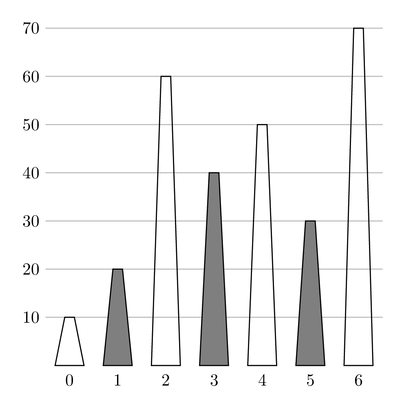
\includegraphics[width=0.42\textwidth]{towers-example.png}
\end{center}

Towers $3$ and $5$ can communicate using tower $4$ as an intermediary, since $40 \leq 50 - 10$ and
$30 \leq 50 - 10$. Towers $1$ and $3$ can communicate using tower $2$ as an intermediary. Towers $1$
and $5$ can communicate using tower $3$ as an intermediary. There is no way to lease more than $3$
towers, therefore the answer is $3$.

For question $1$, with $L = 2$, $R = 2$ and $D = 100$, there is only $1$ tower in the range, thus Pak
Dengklek can only lease $1$ tower. Therefore the answer is $1$.

For question $2$, with $L = 0$, $R = 6$ and $D = 17$, Pak Dengklek can lease towers $1$ and $3$.
Towers $1$ and $3$ can communicate using tower $2$ as an intermediary, since $20 \leq 60 - 17$ and
$40 \leq 60 - 17$. There is no way to lease more than $2$ towers, therefore the answer is $2$.
